\section{Scene construction and exploratory qualification}
\label{app:design}

The shelf and tabletop use the same target meshes, object transforms and cameras in both simulators. Each layout has a block of 32 reserved development seeds. The generator takes the first seed that meets its geometric, framing and duplicate checks. Feasibility trials used separate seeds. A pudding box failed to fit the shelf before collection. The final gelatin box and marker were new target identities relative to the exploratory comparison.

Each of five nominal stops supplies a clear retained reference. The direction of the horizontal translation and the sign of yaw cycle across layouts and stops. In Isaac Sim 6.2.0.0, USD visibility controls whether RTX renders the target. In MuJoCo 3.17.0, the target geoms move to an excluded rendering group. Mesa llvmpipe renders the scene. Both interventions retain the object definition and nominal transform. An enabled flag records the intervention, and native instance masks record visible target pixels. A fully hidden retained object can have an empty visible mask.

Each renderer produces $2304\times1296$ RGB. Lanczos resampling delivers $1200\times675$ inputs. The numeric reference box encloses the scaled, half-open native bounds. The inference call excludes filenames, pairing information, interventions, masks, camera parameters and registration ground truth. Each original verifier independently scored each member of a pair. The evaluator compared both complete decoded images and the box across states and repeated the image check at native resolution.

\begin{figure}[htbp]
  \centering
  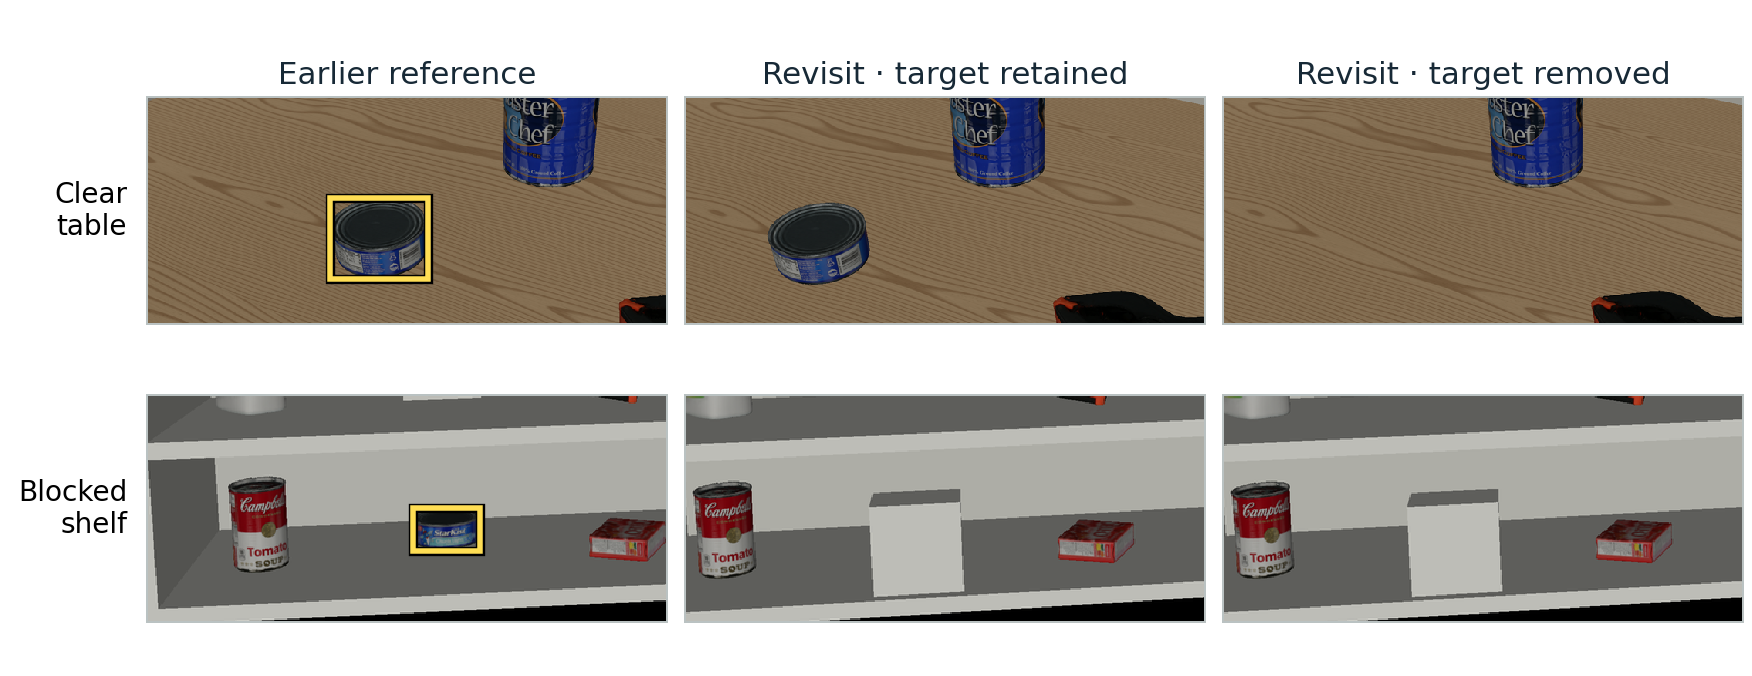
\includegraphics[width=\linewidth]{figures/counterfactual-example.png}
  \caption{Exploratory MuJoCo examples. The outline marks the remembered tuna can. Changing its state alters 12,159 of 810,000 pixels in the tabletop revisit. On the shelf all 810,000 revisit pixels match. The verifier sees one revisit per query. These crops illustrate the intervention.}
  \label{fig:exploratory}
\end{figure}

The exploratory set comprised ten layouts, five per environment, with three camera-motion magnitudes and five stops. At the largest motion, dense geometry found 25/25 clear tabletop removals in each simulator. Homography found 17/25 in Isaac Sim and 16/25 in MuJoCo. Across 1,200 queries, dense geometry gained 113 correct answers and lost 70 relative to homography. It introduced two false deletions of the same retained foam brick at one MuJoCo shelf stop, with the blocker parked and placed. On another fully blocked shelf pair, homography reported removal in both worlds (Figure~\ref{fig:exploratory}). These observations informed the choice of main endpoint and controls.

\section{Verifier settings and capability screens}
\label{app:operating}

\paragraph{Geometry.}
The homography uses a coarse-to-fine enhanced correlation coefficient fit to image edges outside the target neighborhood~\citep{ecc}. Dense geometry estimates camera pose and depth and discards out-of-frame, invalid and depth-inconsistent projections~\citep{vggt,geoscd}. After registration, both methods compare DINOv2 patch features and estimate obstruction from detections and local foreground and background changes~\citep{dinov2,yoloworld}. Registration must pass and local quality must reach 0.30. A similarity of at least 0.70 gives \emph{present}. A similarity of at most 0.60 with obstruction at most 0.40 gives \emph{removed}. All other cases give \emph{unknown}.

\paragraph{Zero-shot Qwen.}
The reader receives two $768\times432$ scene images with the reference box marked, a reference crop, and a warped revisit crop. Each crop fits within $512\times512$ pixels. Although the prompt describes the reference crop as enlarged, preprocessing only downsizes oversized crops. Black pixels in the warped crop denote locations without a mapping. The reader uses greedy decoding and a parser for three literal answers.
The development screen required at least 34/36 correct identical-view answers and 36/40 correct per clear class. Qwen scored 36/36 on unchanged references, 40/40 on clear retained targets, and 40/40 on clear removals. Each simulator supplied 20 of each clear class across nominal and moved cameras. All outputs parsed. The median reference box area was 9,496.5 pixels in the screen and 6,666 on main inputs admitted by registration. The screen contained no hidden targets.

\paragraph{Trained STILL.}
The authors' seed-2 verifier scores the first-token probability of change in red-box crops~\citep{still,still-weights}. Pi3 estimates a projected box from the two RGB images~\citep{pi3}. A crop must have nondegenerate bounds and pass the authors' 0.30 visibility cutoff. We use a constant proposal weight because the target and reference box are supplied. The original SD-V detector also uses proposal confidence. We scored each distinct input tuple once within a split and restored every case to its original position for evaluation.

Development supplied 400 retained and 400 removed queries. Selecting the place threshold for maximum removal F1 gave 0.00071. Selecting it for zero development false deletions gave the conservative value of 0.11916. A third rule uses the geometric mean of the scene and place change scores when a crop exists, and the scene score alone otherwise. Its development-selected threshold was approximately 0.0003872983. The original authors used a threshold calibrated on their own detection scenes. Our binary endpoint counts a withheld deletion on a removed target as a miss. It counts a deletion of a retained target as a false deletion.

\section{Geometric and zero-shot outcomes by simulator}
\label{app:geometry}

\begin{table}[htbp]
  \centering
  \caption{Original three-output verifiers on every main intervention. Each simulator supplied 640 queries, including 320 retained and 320 removed objects. Correct and definite counts include both states. A false presence asserts that a removed object remains.}
  \label{tab:coverage}
  \begin{tabular}{llrrrr}
    \toprule
    Simulator & Verifier & Correct & Definite & \shortstack[r]{False\\ removal} & \shortstack[r]{False\\ presence}\\
    \midrule
    \CoverageRows
    \bottomrule
  \end{tabular}
\end{table}

On clear moved-camera shelf removals, both geometric methods scored 37/40 in Isaac Sim. The score rose from 33/40 to 38/40 in MuJoCo (Figure~\ref{fig:targets}). Across all interventions, dense geometry gained 26 correct answers and lost 16 in Isaac Sim. It gained 38 and lost 27 in MuJoCo. The three original verifiers completed all 3,840 evaluations. An always-abstaining rule gives zero correct answers and zero errors. Always reporting removal gives 80/80 on the clear moved-camera removal endpoint and falsely deletes all 320 retained objects per simulator.

\begin{figure}[htbp]
  \centering
  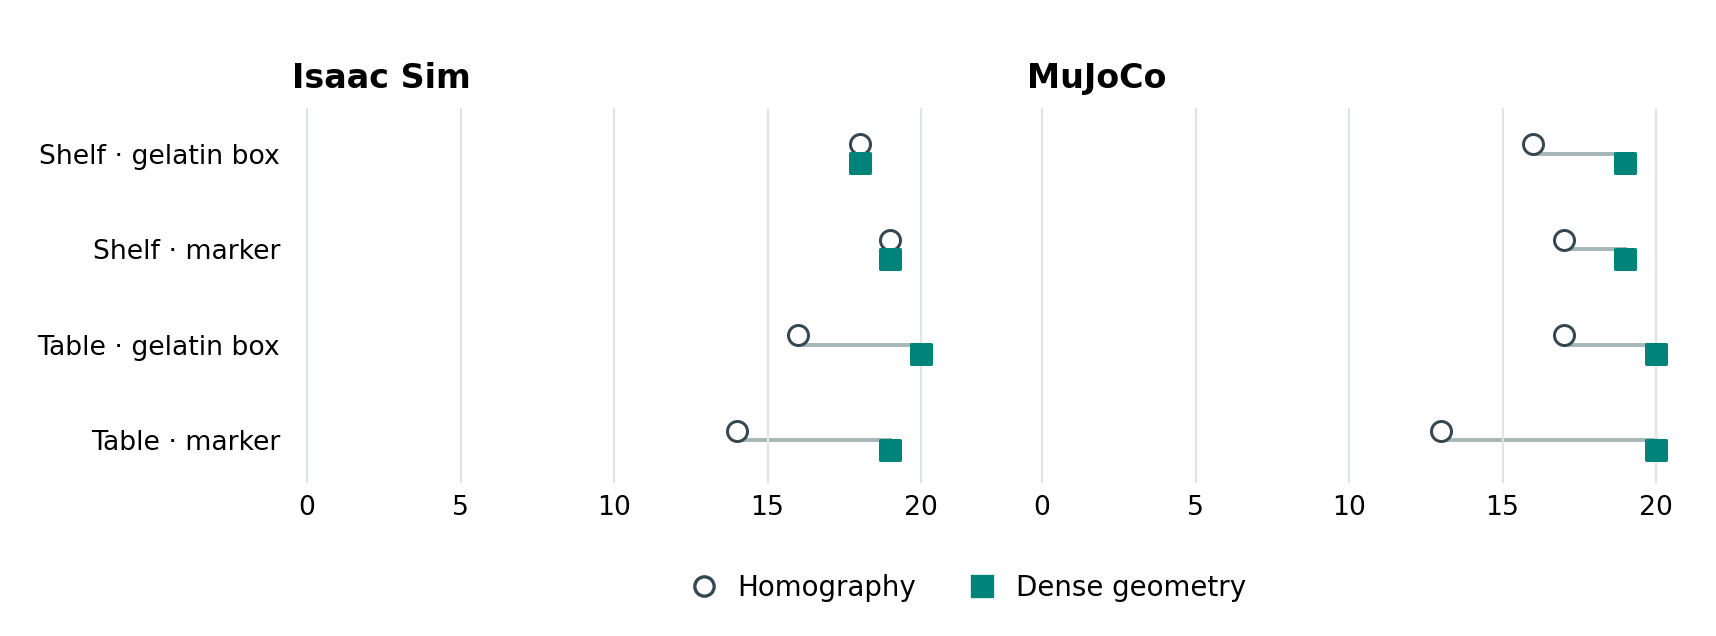
\includegraphics[width=.94\linewidth]{figures/primary-by-target.png}
  \caption{Correct clear removal decisions after camera motion. Each group contains four layouts and five stops per layout. Offset markers show equal counts.}
  \label{fig:targets}
\end{figure}

\begin{table}[htbp]
  \centering
  \caption{Identical retained/removed input pairs by simulator. The last three columns count definite decisions on both twins by the original systems. A dash denotes an empty comparison set.}
  \label{tab:exact}
  \begin{tabular}{lrrrrr}
    \toprule
    Simulator & \shortstack[r]{Identical\\ / all pairs} & \shortstack[r]{Layouts\\ with a pair} & Homography & \shortstack[r]{Dense\\ geometry} & \shortstack[r]{Zero-shot\\ Qwen}\\
    \midrule
    \ExactRows
    \bottomrule
  \end{tabular}
\end{table}

The wide panel completely hid the target at 76/80 placed positions per simulator, and the white box did so at 12/80. None of the 160 parked-blocker pairs per simulator produced identical inputs (Table~\ref{tab:exact}). At MuJoCo shelf PAM05, stop P5, local image quality was 0.737 on the identical pair that dense geometry deleted. Qwen's gate admitted four exact pairs across PAM01, PAM02 and PAM05. All four used the wide blocker, the moved camera, and stop P4 or P5. The gate stopped both members of every other exact pair.

Across all 640 pairs, 176 were completely hidden. Another 402 had full exposure, and four had at least 99.95\% but less than full exposure. The remaining 58 pairs fell between those groups. Of the 51 Qwen false deletions, 29 came from the nominal camera pose. Among the 406 retained targets with at least 99.95\% exposure, Qwen's false deletions by increasing thirds of native silhouette area were 33/135, 10/135 and 4/136. Target identity, layout and size varied together.

Zero-shot Qwen found 80/80 clear moved-camera removals in Isaac Sim and 79/80 in MuJoCo. It also falsely deleted 11 parked-blocker retained targets per simulator. In every parked-blocker retained query, at least 99.96\% of the native silhouette was exposed. Among the 834 queries admitted by the shared gate, Qwen itself abstained twice. Dense geometry found 399/419 removals and erased 2/415 retained objects. It correctly reported \emph{present} on 42 of Qwen's 49 additional false deletions.

\section{What the fixed-camera calibration measures}
\label{app:calibration}

Four separate layouts used a tuna can or foam brick and a side-offset blocker. A base render, two fresh repeats and a distractor-only change accompanied each intervention. The evaluator selected a $7\times7$ patch inside the intersection of the reference mask and the exposed retained-target mask. At least 25 pixels had to qualify. Their mean absolute RGB change had to reach 8 on the 0--255 scale and exceed the larger first-repeat difference by at least 4. Second repeats and distractor changes in each physical state served as negative controls. The screen required zero false triggers, at least eight of ten clear pairs per environment and engine, and a partly visible positive pair in every layout.

The check detected all 20 parked-blocker target interventions per simulator. Each also supplied 13 eligible placed pairs and 132 eligible negative controls. None of these controls triggered. For the remaining 28 of 160 planned negative comparisons per simulator, the evaluator found no eligible patch. Whole-image change exceeded both repeats on 74/80 Isaac Sim and 72/80 MuJoCo distractor manipulations.

Both simulators missed the required yield on partly visible targets. The shelf can in PAC01 produced three fully exposed views, one fully hidden view and one sliver. In MuJoCo, the sliver occupied three native columns and 74 of 6,155 isolated target pixels. No $7\times7$ patch could contain 25 target pixels (Figure~\ref{fig:sliver}). Successful partly visible sites in the other three layouts exposed approximately 48.4\%, 1.9\% and 97.8\% of the silhouette. Only the first falls between 10\% and 90\%.

\begin{figure}[htbp]
  \centering
  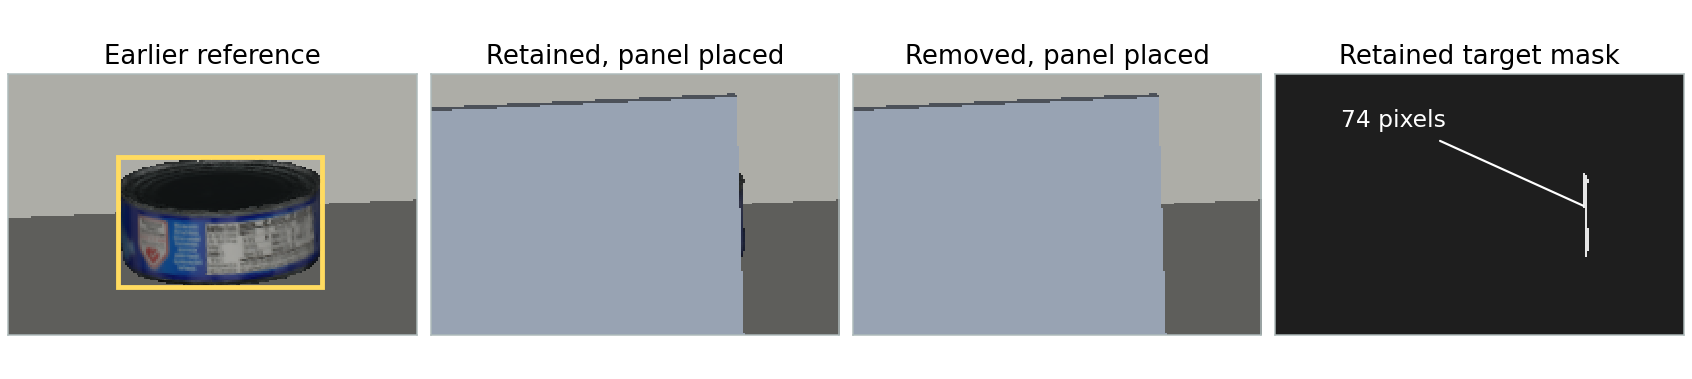
\includegraphics[width=\linewidth]{figures/calibration-sliver.png}
  \caption{Fixed-camera MuJoCo calibration. Only a sliver of the retained can is visible beyond the panel. The right-hand view shows native instance-mask pixels available to the evaluator.}
  \label{fig:sliver}
\end{figure}

Changing the midpoint convention for a half-open box changed seven local contrast values across the two engines. All positive-pair and qualification verdicts stayed the same. Five calibration pairs per simulator had zero visible target pixels. In Isaac Sim the median whole-image mean absolute difference at scoring resolution was 0.321 intensity levels across physical states and 0.326 within same-state repeats. Both medians were zero in MuJoCo.

\paragraph{Why the hidden Isaac Sim images differ.}
We reexamined the 88 fully hidden pairs from the main panel at native resolution. Across the recorded object, shelf and camera fields, only target visibility differed between twins. The blocker mask covered the entire isolated target silhouette at every position. A pixel counted as changed if any RGB channel differed. The median share of changed pixels was 59.2\%, yet the median whole-image mean absolute difference was only 0.293 intensity levels. On 80 unchanged nominal views with the blocker parked, the corresponding median was 0.309. A median of 99.66\% of changed pixels fell outside the target's isolated silhouette, which itself occupies only a small part of the frame.

To check for reproducible local changes, we revisited the five fully hidden calibration views in a post hoc analysis. We divided each original image pair into disjoint $16\times16$ native-pixel tiles and selected the tile with the greatest absolute difference in mean intensity across states. We then evaluated the same tile in two additional archived render pairs at that camera. In four views the tile was brighter after removal on both repeats and lay entirely outside the target and blocker footprints. Its smallest contrast across states exceeded its largest range within either state. The fifth tile reversed sign on one repeat. Figure~\ref{fig:indirect} shows the largest base contrast. A change in indirect lighting is plausible. Capture always rendered the placed, retained state before the placed, removed state, and there was no lighting ablation. These captures cannot identify a specific rendering mechanism or assign a cause to each of the 88 main pairs.

\begin{figure}[htbp]
  \centering
  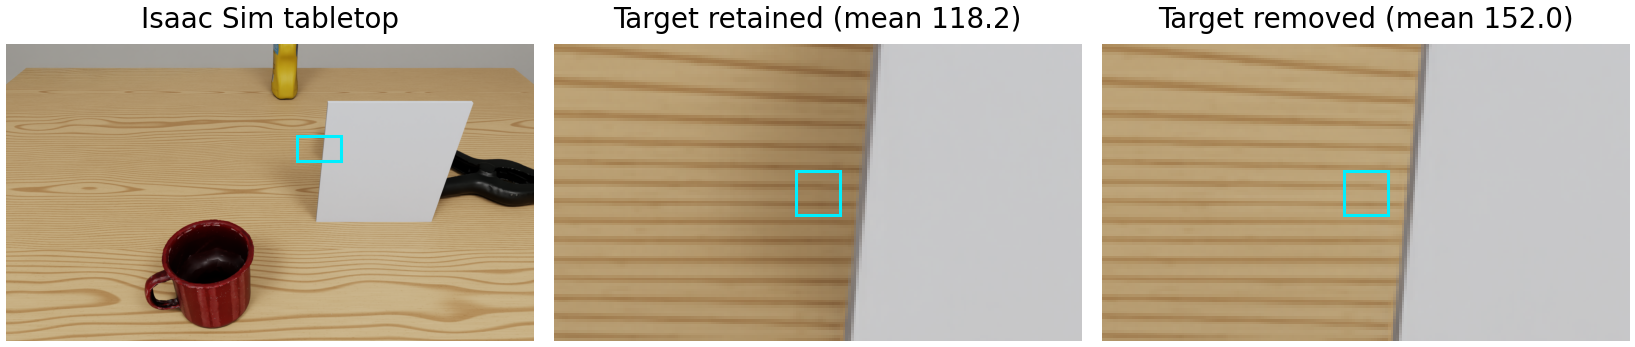
\includegraphics[width=\linewidth]{figures/isaac-hidden-patch.png}
  \caption{Isaac Sim calibration, tabletop PAC04, stop P3. The left outline locates the enlarged crops. The crop outlines mark the same $16\times16$ tile on the exposed tabletop. The tile was 33.9 levels brighter in the removed frame of the base pair and 34.3 and 33.4 levels brighter in the two repeats. The retained foam brick was entirely hidden.}
  \label{fig:indirect}
\end{figure}

\section{Camera and room sensitivity}
\label{app:rooms}

Four previously identified MuJoCo shelf pairs again elicited removal on both states from the zero-shot system at their original camera angles. Rotating each camera in place to level the shelf edge caused registration to reject all four pairs. The language model then received none of them.

Eight fresh service-corridor layouts placed a bottle or drill behind a sliding door. The declared oblique test produced zero double-removal calls on eight identical MuJoCo pairs. A secondary frontal view gave seven on eight pairs. Both camera position and heading changed.

The furnished workshop revisited the same eight layouts after changing the room and door bay. Its declared frontal test gave zero double-removal calls on eight identical MuJoCo pairs. All eight failed registration. Homography classified all 80 open-door controls correctly in each simulator and abstained on every closed-door query. The zero-shot system found all 40 open-door removals per simulator. It falsely deleted an exposed drill on 4/40 retained queries in Isaac Sim and 2/40 in MuJoCo. All six errors occurred on the two added robot camera mounts. The corridor and workshop share layouts, and the furnishing, light and door geometry changed together.

\section{Retrospective replay with a reference at each stop}
\label{app:replay}

The archived panel contains five stops for each combination of simulator, layout, camera-motion level, blocker position and target state. The replay kept any definite homography answer across 640 blocker-placed starts. After an abstention, it took the saved answer from one of the other four stops while holding the other conditions fixed. That answer used the alternate stop's own earlier reference image, target box, and revisit. Across the 1,772 alternate-stop choices for the 443 homography abstentions, both the reference image and its box differed from those at the starting stop.

The starting stop alone gave 196/640 correct decisions (30.6\%). A uniform choice among the alternatives averaged 268.5 (42.0\%). Choosing the alternative with the greatest exposure in the retained twin's evaluator mask gave 292 (45.6\%). The starting and mask-assisted rules each made one false deletion. A ceiling that used both the true state and every alternative's answer reached 319 (49.8\%). These numbers describe a system that stores a reference at each stop and switches to a second reference/revisit pair after abstaining. Evaluating an extra revisit with a single stored reference would require scoring the new revisit against the starting reference and box. The replay used the inspected layouts and omitted travel costs. The proposed study on fresh layouts ended before collection.

\section{Relation to other evaluation designs}
\label{app:related}

PBD-AG tests false absence in robot memory by requiring repeated observable misses based on measured depth~\citep{pbdag}. A robot using SafeVantage can seek evidence from reachable viewpoints under a travel budget~\citep{safevantage}. VA-TAMP obtains observations for actions that depend on uncertain object models~\citep{vatamp}. Our interface fixes a previously identified object, its earlier RGB box and one revisit. With these inputs, certainty about a particular deletion can be tested without choosing a new action.

TRAPSBench pairs answerable and unanswerable physics questions. The Counterfactual Memory Audit varies the available history while fixing the current observation~\citep{trapsbench,cma}. Our intervention holds the supplied history fixed too. SpatialUncertain uses geometry and human screening to evaluate reasoning on occluded views and includes a separate task on perspective and apparent size~\citep{spatialuncertain}. VAD-R studies when models refrain from answering without being prompted to abstain~\citep{vad-r}. Our zero-shot system receives an explicit unknown option. These tasks motivate separating an accurate guess, a supported update and an abstention.

\section{Data and reproducibility}
\label{app:data}

The \href{https://github.com/Adithya-Rajendran/cmpe249-active-verification/releases/tag/scene-memory-audit-v1}{versioned data release} contains the delivered RGB images and their hashes, native renders with evaluator masks, target assignments, case and pair tables, primary protocol, calibration measurements and original scorer outputs. It includes a second analysis implementation from the same project. The visibility analysis and alternate-stop replay reuse these archived cases.

The \href{https://github.com/Adithya-Rajendran/cmpe249-active-verification/blob/a88d89fc5c92f4f18f7a7a1d5947bc59f3b37161/paper/README.md\#reproduce-the-trained-still-comparison}{trained-comparison guide} provides the development and main probabilities, registered boxes, operating points, restored per-query decisions, inference commands and CPU recount. It identifies the exact \href{https://huggingface.co/oran9er/STILL-Qwen3.5-9B/tree/81d9373e1dd9c07c537d5fb2436b36a26a2206b4}{trained STILL} and \href{https://huggingface.co/Qwen/Qwen3.5-9B/tree/c202236235762e1c871ad0ccb60c8ee5ba337b9a}{zero-shot Qwen} model revisions~\citep{still-weights,qwen-weights}. The labels record the simulator intervention. No human annotated support on unequal inputs.
